% !TEX TS-program = pdflatex
% !TEX encoding = UTF-8 Unicode

% Example of the Memoir class, an alternative to the default LaTeX classes such as article and book, with many added features built into the class itself.

\documentclass[12pt,a4paper]{memoir} % for a long document
%\documentclass[12pt,a4paper,article]{memoir} % for a short document
\newif\iftth
\iftth\else
\usepackage{makeidx}
\makeindex
\usepackage[utf8]{inputenc} % set input encoding to utf8
\usepackage{moreverb}
\usepackage{graphicx}
\usepackage{longtable}
\usepackage{pifont}
\usepackage{color}

\usepackage[table]{xcolor}
\usepackage{fancyvrb}
\fi
\usepackage{bbding}
\definecolor{lightblue}{rgb}{0,0,1}
\definecolor{lightred}{rgb}{1,0,0}
\iftth\else
\usepackage{tikz}
\usetikzlibrary{mindmap,trees,snakes}
\fi
%\definecolor{tableShade}{HTML}{F1F5FA}   %iTunes
%\definecolor{tableShade2}{HTML}{ECF3FE} %Finder

%\usepackage{lscape}
\usepackage{pdflscape}
%\usepackage{listings}
%\usepackage{tikz}
%\usepackage{utopia}
%\usepackage[explicit]{titlesec}

%\lstset{language=C,basicstyle=\ttfamily,numbers=left,numberstyle=\tiny}
% Don't forget to read the Memoir manual: memman.pdf

%%% Examples of Memoir customization
%%% enable, disable or adjust these as desired

%%% PAGE DIMENSIONS
% Set up the paper to be as close as possible to both A4 & letter:
%\settrimmedsize{297mm}{210mm}{*} % letter = 11in tall; a4 = 210mm wide
%\setlength{\trimtop}{0pt}
%\setlength{\trimedge}{\stockwidth}
%\addtolength{\trimedge}{-\paperwidth}
%\settypeblocksize{*}{\lxvchars}{1.618} % we want to the text block to have golden proportionals
%\setulmargins{50pt}{*}{*} % 50pt upper margins
%\setlrmargins{*}{*}{1.618} % golden ratio again for left/right margins
%\setheaderspaces{*}{*}{1.618}
%\setheadfoot{\onelineskip}{2\onelineskip}
%\checkandfixthelayout 

%\title{\textsl{A container library for C}}

%\settrimmedsize{297mm}{210mm}{*}
%\setlength{\trimtop}{0pt}
%\setlength{\trimedge}{\stockwidth}
%\addtolength{\trimedge}{-\paperwidth}
\newcommand{\Null}{{\iftth \ NULL \else \footnotesize NULL\  \fi}}
\newcommand{\returns}{\par\noindent\textbf{Returns:}}
\newcommand{\param}[1]{
\texttt{\textsl{#1}}
}
\newcommand{\doerror}[1]{%
\par\noindent
\iftth
{CONTAINER\_ERROR\_#1}
\else
{\footnotesize CONTAINER\_ERROR\_#1}
\fi
}

\iftth\else
\settypeblocksize{634pt}{448.13pt}{*}
\setulmargins{4cm}{*}{*}
\setlrmargins{30mm}{*}{*}
\setmarginnotes{17pt}{51pt}{\onelineskip}
\setheadfoot{\onelineskip}{2\onelineskip}
\setheaderspaces{*}{2\onelineskip}{*}

\checkandfixthelayout
\fi
\newenvironment{ShorterItemize}{
\begin{itemize}
\iftth\else
  \setlength{\itemsep}{1pt}
  \setlength{\parskip}{0pt}
  \setlength{\parsep}{0pt}
\fi
}{\end{itemize}
}
\begin{document}
\chapter{The auxiliary interfaces}
\section{Mask}
A mask is a sequence that contains boolean data used for selection of items in a sequential container. 
It is not specified if a mask is a bit string (i.e. a
strictly boolean array) or an array of chars or other integers used to hold the binary data. In all cases a value of the mask at a given position 
means \textsl{select} if it is different than zero, or \textsl{do not select} if it is zero.

The interface offered by the mask object is very small. Masks can't be resized but they have an allocator to be able to reclaim the
memory they use when created. This allocator will be initialized to the current allocator when the mask is created.
\begin{verbatim}
typedef struct _Mask Mask;
typedef struct tagMaskInterface {
    int (*And)(Mask *src1,Mask *src2);
    int (*Clear)(Mask *m);
    Mask *(*Copy)(const Mask *src);
    Mask *(*Create)(size_t length);
    Mask *(*CreateFromMask)(size_t length,char *data);
    int (*Finalize)(Mask *m);
    int (*Or)(Mask *src1,Mask *src2); 
    size_t (*PopulationCount)(const Mask *m); 
    int (*Set)(Mask *m,size_t idx,int val);
    size_t (*Size)(Mask *);
    size_t (*Sizeof)(Mask *);
} iMask;
\end{verbatim}
\begin{longtable}{|p{3.5cm}|p{11.5cm}|}
\hline
\textbf{Operation}&\textbf{Description}\\\hline 
And&Stores into src1 the result of a logical AND operation between each element of src1 with the corresponding element of src2.\\\hline
Clear &Sets all elements of the mask to zero.\\\hline
Copy&Allocates a new mask and copies the contents of the given one into it.\\\hline
CreateFromMask&Creates a new mask with the specified length and copies the given data into the mask. Each character in the input data is transformed into the mask internal representation. The storage is obtained using the CurrentAllocator pointer.\\\hline
Create&Creates a new mask with the specified length. The storage is obtained using the CurrentAllocator pointer. The data is initialized to zero.\\\hline
Finalize&The memory used by the mask is reclaimed.\\\hline
Not&Stores into src the result of a logical NOT operation: each bit is inverted.\\\hline
Or&Stores into src1 the result of a logical OR operation between each element of src1 with the corresponding element of src2.\\\hline
PopulationCount&Counts the number of entries different from zero in the given mask, returning the sum.\\\hline
Set&Sets the given position to the given value if the value fits in the internal representation of the mask. If not, an implementation defined
conversion occurs.\\\hline
Size&The number of elements in the mask is returned.\\\hline
Sizeof&The number of bytes used by the given mask. If the argument is \Null the number of bytes of the header structure is returned.\\\hline
\end{longtable}


\section{Memory management}
Several interfaces implement different memory allocation strategies. This should give flexibility to the implementations, allowing it to use several memory allocation strategies within the same container.\par
The library starts with the \texttt{default} memory manager, that contains pointers to the default C memory management functions: malloc, free, realloc and calloc. Another memory manager is the \texttt{debug} memory manager that should implement more checking and 
maybe offer hooks to the debugger. The sample
implementation shows how to implement several simple checks, but other implementations can extend this simple interface providing 
much more sophisticated controls.
\begin{verbatim}
typedef struct tagAllocator {
    void *(*malloc)(size_t);
    void  (*free)(void *);
    void *(*realloc)(void *,size_t);
    void *(*calloc)(size_t,size_t);
} ContainerAllocator;
extern ContainerAllocator * CurrentAllocator;
\end{verbatim}

Each of the interface functions corresponds exctly to the specifications of the C language fnctions of the same name. The default memory management interface is initialized with the corresponding C Library functions.



\section{The Heap interface: iHeap}
Some containers can benefit from a cacheing memory manager that manages a stock of objects of the same size. This is not required and not all implementations may provide it. If they do, the interface is:
\begin{verbatim}
    int (*UseHeap)(Container *c);
    ContainerHeap *(*GetHeap)(Container *c);
\end{verbatim}
In the sample implementation, many complex data structures are implemented using a heap. This allows automatically to have an iterator, since for 
looping all elements of the container it suffices to iterate the underlying heap.
The standard interface for the heap is:\index{iHeap}

\begin{verbatim}
typedef struct tagContainerHeapInterface {
   void (*Clear)(ContainerHeap *heap);
   ContainerHeap *(*Create)(size_t ElementSize,
                  const ContainerAllocator *m);
   int (*DeleteIterator)(Iterator *it);
   void (*Finalize)(ContainerHeap *heap);
   int (*FreeObject)(ContainerHeap *heap,void *element);
   ContainerHeap *(*InitHeap)(void *heap,size_t nbElements,
                  const ContainerAllocator *allocator);
   Iterator *(*NewIterator)(ContainerHeap *);
   void *(*NewObject)(ContainerHeap *heap);
   size_t (*Sizeof)(ContainerHeap *heap);
} ContainerHeapInterface;
\end{verbatim}

\begin{longtable}{|p{3.5cm}|p{11.5cm}|}
\hline
\textbf{Operation}&\textbf{Description}\\\hline 
Clear&Releases all memory used by the free list and resets the heap object to its state as it was when created.\\\hline
Create&Creates a new heap object that will use the given memory manager to allocate memory. All elements will have the given size. If the memory manager object pointer is \Null, the object pointed by CurrentAllocator will be used.\\\hline
InitHeap&Initializes the given buffer to a heap header object designed to hold objects of \texttt{ElementSize} bytes. The heap will use the given memory
manager. If the memory manager parameter is \Null the default memory manager is used.

This function supposes that the \texttt{heap} parameter points to a contiguous memory space at least enough to hold a \texttt{ContainerHeap} object.
The size of this object can be obtainer by using the \texttt{iHeap.Size} API with a \Null parameter.
\returns
A pointer to the new ContainerHeap object or \Null if there is an error. Note that the pointer returned can be different from the passed in
pointer due to alignment requirements.\\\hline
newObject&The heap returns a pointer to a new object or \Null if no more memory is left.\\\hline
FreeObject&Adds the given object to the list of free objects, allowing for recycling of memory without new allocations. The element pointer can be \Null.\\\hline
Finalize&Destroys all memory used by the indicated heap and frees the heap object itself.\\\hline
Sizeof&Returns the number of bytes used by the given heap, including the size of the free list. If the argument \texttt{"heap"} is \Null, the result is the size of the heap header structure (i.e. \texttt{sizeof(ContainerHeap)}.\\\hline
\end{longtable}



\section{Pooled memory interface: iPool}
\index{iPool}
Many containers could benefit from a memory pool. A memory pool groups all allocations done in a specific context and can be released in a single call. This allows the programmer to avoid having to manage each single piece of memory like the basic interface.
\begin{verbatim}
typedef struct _tagPoolAllocatorInterface {
    Pool  *(*Create)(ContainerAllocator *m);
    void  *(*Alloc)(Pool *pool,size_t size);
    void  *(*Calloc)(Pool *pool,size_t size);
    void   (*Clear)(Pool *);
    void   (*Finalize)(Pool *);
} PoolAllocatorInterface;
\end{verbatim}
\begin{longtable}{|p{3.5cm}|p{11.5cm}|}
\hline
\textbf{Operation}&\textbf{Description}\\\hline 
Create&Creates a new pool object that will use the given memory manager. If the argument is \Null, the object pointed by the CurrentAllocator will be used.\\\hline
Alloc& Allocates size bytes from the pool pool. If there isn't enough memory to resize the pool  the result is \Null.\\\hline
Calloc&Allocates n objects of size "size" in a single block. All memory is initialized to zero. If there is no memory left it returns \Null.\\\hline
Clear&Reclaims all memory used by the pool and leaves the object as it was when created.\\\hline
Finalize&Reclaims all memory used by the pool and destroys the pool object itself.\\\hline

\end{longtable}




\section{Error handling Interface: iError}
The "iError" interface provides a default strategy for handling errors. The "RaiseError" function will be used as the default error function within the creation function for all containers that support a per container instance error function.
\index{iError}
\begin{verbatim}
typedef (*ErrorFunction)(const char *,int,...);
typedef struct {
  void        (*EmptyErrorFunction)(const char *fname,int code,...);
  int         (*NullPtrError)(const char *);
  void        (*RaiseError)(const char *fname,int code,...);
  ErrorFunction (*SetErrorFunction)(ErrorFunction);
  const char *(*StrError)(int errorCode);
} ErrorInterface;
\end{verbatim}
\begin{longtable}{|p{3.5cm}|p{11.5cm}|}
\hline
\textbf{Operation}&\textbf{Description}\\\hline 
EmptyErrorFunction&This function can be used to ignore all errors within the library. It does nothing.\\\hline
NullPtrError&Calls \texttt{RaiseError}, then returns \texttt{CONTAINER\_ERROR\_BADARG}\\\hline
RaiseError&The parameter "fname" should be the name of the function where the error occurs. The "errcode" parameter is a negative error code. See \ref{errorcodes}. Other parameters can be passed depending on the error. \\\hline

\end{longtable}

\subsection{Error codes}
\label{errorcodes} 
The error codes defined by this specification are:
\index{error-codes}
\begin{itemize}
\item
\doerror{BADARG} One of the parameters passed to a function is invalid.
\item
\doerror{NOMEMORY} There is not enough memory to complete the operation.
\item
\doerror{INDEX} The index is out of bounds. 
The library passes extra parameters when this error is invoked: the \verb,container, pointer, and a \verb,size_t, containing the
the out of bounds index.
\item
\doerror{READONLY} The object is read-only and the operation would modify it 
\item
\doerror{INTERNAL} Unspecified error provoked by a problem in the implementation.
\item
\doerror{OBJECT\_CHANGED} A change in the underlying object has invalidated an iterator. 
\item
\doerror{FILE\_READ} Input error in a stream.
\item
\doerror{FILE\_WRITE} Output error in a stream.
\item
\doerror{CONTAINER\_FULL} Implementations can limit the maximum number of elements a container can hold. This error indicates that the limit is reached.
\item
\doerror{BADPOINTER} The debug implementation of \texttt{free()} has discovered an incorrect pointer attempting to be freed
\item
\doerror{BUFFEROVERFLOW} The debug implementation of \texttt{free()} discovered a buffer overflow.
\item
\doerror{WRONGFILE} You are trying to read a container from a stream that has no such container saved
\item 
\doerror{DIVISION\_BY\_ZERO} The library has detected an attempt to divide by zero.
\item
\doerror{OVERFLOW} An overflow was detected in an arithmetic operation. Implementations are encouraged to detect overflow in all operations that
can generate one and report it through this error.
\item
\doerror{BADMASK} The mask given to a \verb,Select, or \verb,SelectCopy, operation is of a different length than the length of the associated
container. The library passes two pointers to the error function: The first to the container and the second to the mask.
\item
\doerror{NOENT} The library wants to open a file that doesn't exist or is not readable. A pointer to the name of the file is passed to the error function
\end{itemize}




\section{The iterator interface}
The iterator object exposes at least the functions "GetFirst", for initializing the loop, and "GetNext", for getting the next element in the sequence. 
The functions "NewIterator" and "deleteIterator" are specific to each container interface even if they all have the same syntax.
\begin{verbatim}
typedef struct _Iterator {
    void *(*GetNext)(Iterator *);
    void *(*GetPrevious)(Iterator *);
    void *(*GetFirst)(Iterator *);
    void *(*GetCurrent)(Iterator *);
    void *(*GetLast)(Iterator *);
    void *(*Seek)(Iterator *it,size_t pos);
    int (*Replace)(Iterator *it, void *data, int direction);
} Iterator;
\end{verbatim}
\begin{longtable}{|p{3.5cm}|p{11.5cm}|}
\hline
\textbf{Operation}&\textbf{Description}\\\hline 
GetCurrent&Returns the element at the cursor position.\\\hline
GetFirst&This function initializes the given iterator to the first element in the container. For sequential operators this is the element with index zero. In 
associative operators which element is the first is implementation defined and can change if elements are added or removed from the container.\\\hline
GetNext&Positions de cursor at the next element and returns a pointer to its contents. If the iterator is at the end of the container the result is \Null 
and the iterator remains at the last position, a subsequent call to GetCurrent returns the last element.\\\hline
GetPrevious&Positions de cursor at the previous element and returns a pointer to its contents. If the pointer is at the beginning of the container the
result is \Null and the iterator remains at the beginning, a subsequent call to GetCurrent will return the first element of the container.


This function is meaningful only in sequential containers. Its existence in associative containers is implementation defined. Even in sequential 
containers, it can be very expensive to find a previous element, for instance in single linked lists.\\\hline
GetLast&Positions the cursor at the last element and returns a pointer to it. Returns \Null if the container is empty.  If the container is read-only, a pointer 
to a copy of the element is returned.\\\hline
Seek&Positions the given iterator at the indicated position and then returns a pointer to the element's data at that position. 
If the position is bigger than the last element of the container, the last element position will be used.\\\hline
Replace&Replaces the current object pointed by the given iterator with the new data. If the\param{data} argument is \Null the element is erased from the
container. If the \param{direction} parameter is different from zero, in sequential containers the iterator will point to the next element,
otherwise it will point to the previous element. In associative containers this parameter is ignored and the iterator is always set to the next
element, if any.\\\hline
\end{longtable}


\section{The observer interface}
In its general form, the observer design pattern can be defined as a one-to-many dependency between objects so that when one object 
changes state, all its dependents are notified and updated automatically. 

When a container changes its state, specifically when elements are added or removed, it is sometimes necessary to update relationships that 
can be very complex.
The observer interface is designed to simplify this operation by allowing the container to emit \textsl{notifications} to other objects that have 
previously manifested interest in receiving them by \textsl{subscribing} to them. In general notifications are sent only when one of the defined
operations for a container occur, mostly operations that change the number of elements.

This interface then, establishes a relationship between two software entities:
\begin{enumerate}
\item The container, that is responsible for sending the notifications when appropriate
\item The receiver, that is an unspecified object represented by its callback function that is called when a change occurs that matches the
notifications specified in the subscription.
\end{enumerate}

Since this relationship needs both objects, it will be finished when either object goes out of scope or breaks the relationship for whatever 
reason. Both objects can unsubscribe (terminate) their relationship.
\subsection{Caveats}
\begin{itemize}
\item
It is in general a bad idea to modify the object being observed during a notification since this could trigger other notification
messages. Implementations are not required to avoid this situation that is the responsibility of the programmer. Contrary to the iterator interface
no error is issued when a possible infinite loop is started. Implementations may catch the error by limiting the number of recursive
invocations of this interface but they are not required to do so.
\item
Since all messages sent by the containers have different type of information in the same two arguments that each message is associated with,
there is no possible compile time control of the usage of the received pointers or numbers. The observer function must correctly 
discriminate between the different messages it can receive.
\end{itemize}
\begin{verbatim}
typedef void (*ObserverFunction)(const void *ObservedObject,
                                 unsigned Operation, 
                                 void *ExtraInfo[]);

typedef struct tagObserverInterface {
    int (*Subscribe)(void *ObservedObject, 
                     ObserverFunction callback, unsigned Operations);
    int (*Notify)(const void *ObservedObject,unsigned operation,
                  void *ExtraInfo1,void *ExtraInfo2);
    size_t (*Unsubscribe)(void *ObservedObject,
                          ObserverFunction callback);
} ObserverInterface;
extern ObserverInterface iObserver;
\end{verbatim}
\begin{longtable}{|p{3.5cm}|p{11.5cm}|}
\hline
\textbf{Operation}&\textbf{Description}\\\hline 
Subscribe&Establishes the relationship between the observed object (argument 1) and the observer, represented by its callback (argument 2).
The third argument establishes which operations are to be observed.
This operation performs an allocation to register the relationship in the observer interface tables, therefore it can fail with an out of memory 
condition.\\\hline
Notify&Used by the container to send a message to the receiver callback. The arguments correspond roughly to the arguments the callback
function will receive. "Notify" will call all the objects that are observing \texttt{ObservedObject} and that have subscribed to one of the 
operations
specified in the \texttt{Operation} argument. This implies a search through the observer interface table, and possibly several calls, making
this function quite expensive. The time needed is roughly proportional to the number of registered callbacks and the complexity of the callbacks
themselves.\\\hline
Unsubscribe&Breaks the relationship between the observed object and the observer. There are several combinations of both arguments:
\begin{itemize}
\item The \texttt{ObservedObject} argument is \Null. This means that the \texttt{callback} object wants to break its relationship to all objects it is
observing. The observer interface will remove all relationships that contain this callback from its tables.
\item The \texttt{callback} argument is \Null. This means that the given \texttt{ObservedObject} is going out of scope and wants to break all
relationships to all its observers. The interface removes from its tables all relationships that have this object as the observed object.
This happens normally immediately after the notification \texttt{FINALIZE} is sent.
\item If both \texttt{callback} and \texttt{ObservedObject} are non \Null, only the matching relationship will be removed from the tables.
\end{itemize}\\\hline

ObserverFunction&This function will be called by the interface when a notification is received for an observed object.  The call happens after all arguments have been processed, the actual work of the function is finished (when adding an object) or not yet done (when destroying an object). 
The container is in a consistent state. For the callbacks that are called when an object is deleted from a
container the call happens before any call to \texttt{free()} and before any call to a destructor (if any) is done. For the calls that add an object
the callback is called after the container has been modified. 

Arguments:
\begin{enumerate}
\item \texttt{ObservedObject}: Specifies the object that sends the notification, i.e. the container
that has the subscription. It is assumed that this container conforms to the \texttt{iGeneric} interface.
\item \texttt{Operation}: The operation that provoked the notification. Since it is possible to subscribe to several operations with only one callback function,
this argument allows the callback to discriminate between the operation notifications.
\item \texttt{ExtraInfo}: This argument is specific to each operation and conveys further information for each operation.
\end{enumerate}

None of the arguments will be ever \Null or zero.\\\hline
\end{longtable}
\subsection{Notification messages}
\begin{longtable}{|p{2cm}|p{6.5cm}|p{6cm}|}
\hline
{\textbf{Operation}} &
{\textbf{Argument 1}} &
{\textbf{Argument 2}}\\
\hline
\endfirsthead

%This is the header for the remaining page(s) of the table...

\multicolumn{3}{c}{{\tablename} \thetable{} -- Continued} \\[0.5ex]
%\hline 

{\textbf{Operation}} &
{\textbf{Argument 1}} &
{\textbf{Argument 2}}\\
\hline
\endhead
Add&Pointer to the new object& \Null or slice specs if any\\ \hline
AddRange&A \texttt{size\_t} with the number of objects added&Pointer to a table of \textsl{n} elements that were added\\ \hline
Append&A pointer to the object being appended. It is of the same type as the object emitting the notification&  \Null\\ \hline
Clear&Pointer to the container being cleared& \Null\\ \hline
Copy&Pointer to the copy of the container& \Null\\ \hline
Erase&Pointer to the object being deleted. The object is still valid& \Null\\ \hline
EraseAt&Pointer to object being deleted&Position (as size\_t)\\ \hline
Finalize& \Null& \Null\\ \hline
Insert&Pointer to the new object being inserted&A \texttt{size\_t} with the position of the object being inserted if applicable\\ \hline
InsertIn&Pointer to the object being inserted, that has the same type as the object sending the notification& \Null\\ \hline
Pop&Pointer to the object being popped& \Null\\ \hline
Push&Pointer to the object being pushed& \Null\\ \hline
ReplaceAt&Pointer to the old value&Pointer to the new value\\ \hline
\end{longtable}
\chapter{The containers}
\index{List}
\section{The List interfaces: iList, iDlist}
The list container appears in two flavors: 
\begin{itemize}
\item
single linked lists: the iList type
\item
double linked lists the iDlist type
\end{itemize}
The space overhead of single linked lists is smaller at the expense of more difficult access to the elements. It is up to the application programmer to decide which container fits best in his/her application
\footnote{
The single linked list container corresponds to the C++ STL \texttt{forward\_list}.
}.

It is often more efficient to get the next element from a list starting with the previous element instead of searching the whole list starting from the beginning. For this, the list and the Dlist containers provide:
\begin{ShorterItemize}
\item \verb,FirstElement, Start of the list
\item \verb,LastElement, End of the list
\item \verb,NextElement, Returns a pointer to the next element
\item \verb,PreviousElement, Only in double linked lists. Returns a pointer to the previous element.
\item \verb,ElementData, Extracts a pointer to the element data 
\item \verb,SetElementData, Modifies one element of the list.
\item \verb,Advance, Returns the data of an element and advances the given pointer in one operation.
\item \verb,MoveBack, Returns the data of an element and moves back the pointer one element. This operation is available only in double linked lists.
\end{ShorterItemize}

These operations can't be done in a read-only list.

The exact layout of the \verb,ListElement, structure is undefined and private to each implementation. This is the reason for providing the \verb,ElementData, function: it hides the exact position and layout of the data from user code, that remains independent from implementation details.

The interfaces of both containers are very similar. Double linked lists support all functions in single linked ones, and add a few more. To avoid unnecessary repetition we document here all the single linked list interface, then only the functions that the Dlist interface adds to it.
\begin{verbatim}
typedef struct tagListInterface {
   int (*Add)(List *L,const void *newval);
   int (*AddRange)(List *L, size_t n,const void *data);
   void *(*Advance)(ListElement **pListElement);
   int (*Append)(List *l1,List *l2);
   int (*Apply)(List *L,int(Applyfn)(void *,void *),void *arg);
   void *(*Back)(const List *l);
   int (*Clear)(List *L);
   int (*Contains)(const List *L,const void *element);
   List *(*Copy)(const List *L);
   int (*CopyElement)(const List *list,size_t idx,void *OutBuffer);
   List *(*Create)(size_t element_size);
   List *(*CreateWithAllocator)(size_t elementsize,
         const ContainerAllocator *mm);
   int (*DeleteIterator)(Iterator *);
   int (*Equal)(const List *l1,const List *l2);
   int (*Erase)(List *L,const void *);
   int (*EraseAll)(List *l,const void *);
   int (*EraseAt)(List *L,size_t idx);
   int (*EraseRange)(List *L,size_t start,size_t end);
   int (*Finalize)(List *L);
   ListElement *(*FirstElement)(List *l);
   void *(*Front)(const List *l);
   const ContainerAllocator *(*GetAllocator)(const List *list);
   void *(*GetElement)(const List *L,size_t idx);
   void *(*GetElementData)(ListElement *le);
   size_t (*GetElementSize)(const List *l);
   unsigned (*GetFlags)(const List *L);
   ContainerHeap *(*GetHeap)(const List *l);
   List *(*GetRange)(const List *l,size_t start,size_t end);
   int (*IndexOf)(const List *L,const void *SearchedElement,
        void *ExtraArgs,size_t *result);
   List *(*Init)(List *aList,size_t element_size);
   int (*InitIterator)(List *L,void *buf);
   List *(*InitWithAllocator)(List *aList,size_t element_size,
         const ContainerAllocator *mm);
   List *(*InitializeWith)(size_t elementSize,size_t n,
         const void *data);
   int (*InsertAt)(List *L,size_t idx,const void *newval);
   int (*InsertIn)(List *l, size_t idx,List *newData);
   ListElement *(*LastElement)(List *l);
   List *(*Load)(FILE *stream, ReadFunction loadFn,void *arg);
   Iterator *(*NewIterator)(List *L);
   ListElement *(*NextElement)(ListElement *le);
   int (*PopFront)(List *L,void *result);
   int (*PushFront)(List *L,const void *str);
   int (*RemoveRange)(List *l,size_t start, size_t end);
   int (*ReplaceAt)(List *L,size_t idx,const void *newval);
   int (*Reverse)(List *l);
   int (*RotateLeft)(List *l, size_t n);
   int (*RotateRight)(List *l,size_t n);
   int (*Save)(const List *L,FILE *stream, SaveFunction saveFn,
        void *arg);
   int (*Select)(List *src,const Mask *m);
   List *(*SelectCopy)(const List *src,const Mask *m);
   CompareFunction (*SetCompareFunction)(List *l,CompareFunction fn);
   DestructorFunction (*SetDestructor)(List *v,DestructorFunction fn);
   int (*SetElementData)(List *l, ListElement *le,void *data);
   ErrorFunction (*SetErrorFunction)(List *L,ErrorFunction);
   unsigned (*SetFlags)(List *L,unsigned flags);
   size_t (*Size)(const List *L);
   size_t (*Sizeof)(const List *l);
   size_t (*SizeofIterator)(const List *);
   ListElement *(*Skip)(ListElement *l,size_t n);
   int (*Sort)(List *l);
   List *(*SplitAfter)(List *l, ListElement *pt);
   int (*UseHeap)(List *L, const ContainerAllocator *m);
} ListInterface;
\end{verbatim}

\par\noindent
\subsection{General remarks}
Lists are containers that store each element in a sequence, unidirectionally (single linked lists) or bidirectionally (double linked lists).
The advantage of linked lists is their flexibility. You can easily and with a very low cost remove or add elements by manipulating the links between the elements. Single linked lists have less overhead than their double linked counterparts (one pointer less in each node), but they tend to use a lot of computer power when inserting elements near the end of the list: you have to follow all links from the beginning until you find the right one.

The list nodes themselves do not move around, only their links are changed. This can be important if you maintain pointers to those elements. Obviously, if you delete a node, its contents (that do not move) could be recycled to contain something else than what you expect.

The iList interface consists (as all other interfaces) of a table of function pointers. The interface describes the behavior of the List container.

The stack operations push and pop are provided with PushFront and PopFront because they have a very low cost, insertion at the start of a single linked list is very fast. PushBack is the equivalent of the \verb,Add, operation, but PopBack would have a very high cost since it would need going through all the list. 

The list container features in some implementations a per list error function.  This is the function that will be called for any errors, except in  
cases where no list object exists: the creation function, or the error of getting a \Null pointer instead of a list pointer. In those cases the general 
iError interface is used, and iError.RaiseError is called. The default value of the list error function is the function iError.RaiseError at the moment 
the list is created.

Other implementations of this interface may specialize list for a certain category of uses: lists of a few elements would try to reduce overhead by 
eliminating a per list error function and replace it with the standard error function in iError, for instance, eliminating their fields in the header. 
If the read-only flag support is dropped, the whole "Flags" field can be eliminated. In such an implementation, the SetFlags primitive would always 
return an error code.

The sample implementation of the list container supports the following state flags:
\begin{verbatim}
#define CONTAINER_READONLY          1
\end{verbatim}
If this flag is set, no modifications to the container are allowed, and the Clear and Finalize functions will not work. Only copies of the data are 
handed out, no direct pointers to the data are available.
\begin{verbatim}
#define CONTAINER_SORTED_FRONT      2
#define CONTAINER_SORTED_BACK       4
\end{verbatim}
If this flag is set, the container is maintained always in sorted order, with the biggest element at the index zero for \verb,CONTAINER_SORTED_FRONT,
or with the biggest element at the end if \verb,CONTAINER_SORTED_BACK, is set. It is an error if both flags are set, and the results in that  case
are implementation defined.
\subsubsection{Specializations}
All "specialized" containers share the same interface with the following exceptions:
\begin{ShorterItemize}
\item The functions where a \verb,void *, to the element data is passed or where a \verb,void *, is the result of the operation are replaced with the 
actual data type of the specialization. For instance the \verb,GetElement, API instead of returning a void pointer returns a pointer to the specific 
data type: an 
integer for \verb,intList,, a double for \verb,doubleList, etc.
\item The creation and initialization functions that construct a new container receive one argument less than its generic counterparts since the
size of each element is fixed.

To make things clear and to save work from the library user some specializations are delivered with the sample implementation to show how a
\textsl{file templated} container looks like.
\end{ShorterItemize}
\begin{center}
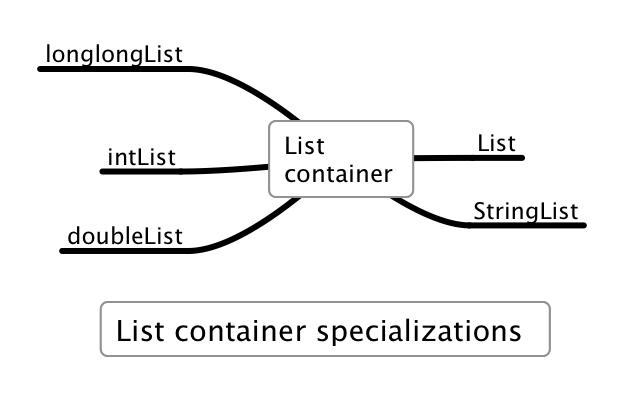
\includegraphics[scale=0.625]{ListContainerSpecializations.png}
\end{center}
In the right side of the drawing we see the generic list container using generic pointers (\verb,void *,) and the stringlist container. Strings are 
special because in C their length is the result of a function call instead of being fixed like other data types.

In the left side, we see three specialized containers for some numeric data types. Those containers are generated using two types of source files:
\begin{ShorterItemize}
\item Parameter files: They define the data type and some other parameters like the comparison expression.
\item Templated files: They implement the specialized container. The pre-processor does the editing work on the templated file to yield several 
different type definitions. Using this interface has the advantage of ensuring compile time checking of the arguments to the API, what is not
possible using generic pointers.
\end{ShorterItemize}
\begin{longtable}{|p{3.5cm}|p{11.5cm}|}
\hline
\textbf{Operation}&\textbf{Description}\\\hline 
Add&Adds the given element to the container. In its generic form it is assumed that "data" points to a contiguous memory area of at least ElementSize 
bytes. In its specialized form the data is passed by value. Returns a value greater than zero if the addition of the element to the list completed 
successfully, a negative error code otherwise.\\\hline
Advance&Given the address of a pointer to an element, it returns a pointer to the data stored into that element and writes the address of the next element
into its argument \verb,ppElement,. If ppElement is\Null it returns\Null. If \verb,*ppElement, is\Null it also returns\Null, and obviously there 
is no advancing done.\\\hline
AddRange&Adds the n given elements to the end of the container. It is the same operations as the PushBack operation. It is assumed that "data" points to a 
contiguous memory area of at least n*ElementSize bytes. If \textsl{n} is zero no error is issued even if the array pointer or the data pointer are 
\Null.\\\hline
Append&Appends the contents of list2 to list1 and destroys list2.\\\hline
Apply&Will call the given function for each element of the list. The first argument of the callback function receives an element of the list. The second argument of the callback is the arg argument that the Apply function receives and passes to  the callback. This way some context can be passed to the callback, and from one element to the next.
Note that the result of the callback is not used. This allows all kinds of result types to be accepted after a suitable cast.
If the list is read-only, a copy of the element will be passed to the callback function.\\\hline
Back&Returns the last element of the given list or \Null if the list is empty.\\\hline
Clear&Erases all stored data and releases the memory associated with it. The list header will not be destroyed, and its contents will be the same as when the list was initially created. It is an error to use this function when there are still active iterators for the container.\\\hline
Contains&Returns one if the given data is stored in the list, zero otherwise. The "data" argument is supposed to point to an element at least ElementSize bytes. The list's comparison function is used for determining if two elements are equal. This comparison function defaults to memcmp.\\\hline
Copy&A shallow copy of the given list is performed. Only ElementSize bytes will be copied for each element. If the element contains pointers, only the pointers are copied, not the objects they point to. The new memory will be allocated using the given list's allocator.\\\hline
CopyElement&Copies the element data at the given position into the given buffer, assuming that at least ElementSize bytes of storage are available at the position pointed by the output buffer. The main usage of this function is to access data in a read only container for later modification.\\\hline
Create&The creation function returns an empty List container, initialized with all the default values.
The current memory manager is used to allocate the space needed for the List header. The list is supposed to contain elements of the same size. If the elements you want to store are of different size, use a pointer to them, and create the list with sizeof(void *) as the size parameter.\\\hline
deleteIterator&Reclaims the memory used by the given iterator object\\\hline
Equal&Compares the given lists using the list comparison function of either list1 or list2 that must compare equal. If the list differ in their length, flags, or any other characteristic they compare unequal. If any of their elements differ, they compare unequal.
If both list1 and list2 are \Null they compare equal. If both list1 and list2 are empty they compare equal.\\\hline
EraseRange&Removes from the list the given range, starting with the \texttt{start} index, until the element before the \texttt{end} index. If \texttt{end}
is greater than the length of the list, it will be 'rounded' to the length of the list.\\\hline
EraseAt&Removes from the list the element at the given position.\\\hline
EraseRage&Removes from the list the given range, starting with the \texttt{start} index, until the element before the \texttt{end} index. If \texttt{end}
is greater than the length of the list, it will be 'rounded' to the length of the list.\\\hline
Finalize&Reclaims all memory used by the list, including the list header object itself.\\\hline
FirstElement&Finds the first element of the list and returns a pointer to it. This is a pointer to the element, \textbf{not} to the data stored at that element.
It is an error to attempt to use this function with a read-only list. \\\hline
Front&Returns a pointer to the first element of the given list or \Null if the list is empty.\\\hline
GetAllocator&Returns the list's allocator object. If the list pointer is \Null it returns \Null.\\\hline
GetElementSize&Retrieves the size of the elements stored in the given list. Note that this value can be different than the value given to the creation function because of alignment requirements.\\\hline
GetElement&Returns a read only pointer to the element at the given index, or \Null if the operation failed.  This function will return \Null if the list is read only.
Use the CopyElement function to get a read/write copy of an element of the list.\\\hline

\end{longtable}
\end{document}